\documentclass[10pt,xcolor=dvipsnames]{beamer}

\usetheme{CambridgeUS}
\usepackage[utf8x]{inputenc}
\usepackage{default}
\usepackage{graphicx}
\usepackage{epstopdf}
\usepackage{color}
\usepackage{amssymb,amsmath,amsfonts}
\usepackage{tikz}

\setbeamertemplate{navigation symbols}{}
\setbeamertemplate{itemize items}[square]
\setbeamertemplate{itemize subitem}[triangle]
\setbeamercolor{itemize item}{fg=darkred!80!gray}
\setbeamercolor{itemize subitem}{fg=darkred!80!gray}
\setbeamertemplate{title page}[default][colsep=-4bp,rounded=true]
\setbeamertemplate{blocks}[default]
\setbeamercolor{block title}{bg=darkred!80!black,fg=white}
\setbeamercolor{block body}{bg=gray!15!white,fg=black}

\setbeamercolor{blank}{bg=white,fg=white}
\setbeamercolor{note}{fg=white,bg=darkred!80!black}

\newenvironment<>{emphblock}{
 \begin{actionenv}%
  \def\insertblocktitle{\vspace{-1.25ex}}
  \par
  \mode<presentation>{
   \setbeamercolor{block title}{}
   \setbeamercolor{block body}{fg=white,bg=darkred!80!black}
   \setbeamercolor{itemize item}{fg=white,bg=darkred!80!black}
   \setbeamertemplate{itemize item}[square]
  }
  \usebeamertemplate{block begin}}
 {\par\usebeamertemplate{block end}\end{actionenv}
}

\title[Pedestal Structure in I-Mode]{ELM Suppression and Pedestal Structure\\ in I-Mode Plasmas on Alcator C-Mod\\\vspace{-1em}}
\author[JR Walk]{John Walk}
\institute[MIT PSFC]{MIT Plasma Science and Fusion Center}
\date[7/22/14]{Thesis Defense -- 22 July 2014}

\graphicspath{{/home/jrwalk/Documents/CMod/common_graphics/}{E:/Libraries/Documents/Schoolwork/graphics/}}

\begin{document}

%%%%%%%%%%%%%%%%%%%%%%%%%%%%%%%%%%%%%%%%%%%%%%%%%%%%%%%%%%%%%%%%%%%%%

\begin{frame}

 \titlepage
 \begin{tikzpicture}[overlay]
  \node[anchor=east,xshift=-2ex,yshift=3ex] at (current page.south east) {\includegraphics[height=2cm]{cmodlogo.eps}};
 \end{tikzpicture}
 
\end{frame}

%%%%%%%%%%%%%%%%%%%%%%%%%%%%%%%%%%%%%%%%%%%%%%%%%%%%%%%%%%%%%%%%%%%%%

\begin{frame}{Thank you to...}

\large
\begin{itemize}
 \item The thesis committee: JW Hughes, DG Whyte, AE White, JP Freidberg
 \vspace{0.5em}
 \item The I-mode crew: AE Hubbard, JL Terry, I Cziegler, A Dominguez, SG Baek, C Theiler, RM Churchill, ML Reinke, JE Rice...
 \vspace{0.5em}
 \item Physops: R Granetz, S Shiraiwa, S Wolfe, S Wukitch...
 \vspace{0.5em}
 \item C-Mod operations, engineering, researchers and techs
 \vspace{0.5em}
 \item PSFC grad students, past and present
 \vspace{0.5em}
 \item Family and friends
 \vspace{0.5em}
 \item the audience!
\end{itemize}

\end{frame}

%%%%%%%%%%%%%%%%%%%%%%%%%%%%%%%%%%%%%%%%%%%%%%%%%%%%%%%%%%%%%%%%%%%%%

\begin{frame}{Outline}

\only<1>{\begin{itemize}
 \large
 \item \textbf{Context \& Motivation}
 \begin{itemize}
  \large 
  \item High-performance regimes
  \item Pedestal physics
  \item Introduction to I-mode
 \end{itemize}
 \vspace{0.5em}
 \item \textbf{Pedestal Modeling \& Theory}:
 \begin{itemize}
  \large
  \item Peeling-ballooning MHD stability
  \item Kinetic-ballooning mode turbulence
 \end{itemize}
 \vspace{0.5em}
 \item \textbf{ELMy H-mode physics}\footnote{JR Walk \emph{et al.}, \emph{Nuclear Fusion} \textbf{52} (2012)}
 \begin{itemize}
  \large
  \item EPED Modeling on C-Mod
 \end{itemize}
\end{itemize}}

\only<2->{\begin{itemize}
 \large
 \item \textbf{I-Mode Pedestals \& Global Performance}\footnote{JR Walk \emph{et al.}, \emph{Physics of Plasmas} \textbf{21} (2014)}
 \begin{itemize}
  \large
  \item Pedestal response to fueling, heating power
  \item Pedestal widths and gradients
  \item Global performance and confinement scalings
 \end{itemize}
 \vspace{0.5em}
 \item \textbf{I-Mode Pedestal Stability}
 \begin{itemize}
  \large
  \item P-B MHD, KBM modeling
  \item ELM characterization
 \end{itemize}
 \vspace{0.5em}
 \item \textbf{Summary, Future Work, \& Questions}
\end{itemize}}

\end{frame}

%%%%%%%%%%%%%%%%%%%%%%%%%%%%%%%%%%%%%%%%%%%%%%%%%%%%%%%%%%%%%%%%%%%%%

\begin{frame}{The problem...}

 \large
 By default (``L-mode''), rapid transport of energy and particles from plasma driven by turbulence
 
 \begin{itemize}
  \item and energy transport gets \emph{worse} with more heating power!
  \item need very strong magnetic field and/or large machine size to overcome poor plasma performance
 \end{itemize}
 
\begin{emphblock}{}
  \centering
  L-mode likely not suitable for (economical) power plant development.
 \end{emphblock}

\end{frame}

%%%%%%%%%%%%%%%%%%%%%%%%%%%%%%%%%%%%%%%%%%%%%%%%%%%%%%%%%%%%%%%%%%%%%

\begin{frame}{The solution?}
 \large
 Under right conditions, plasma forms ``transport barrier'' in edge, with steep gradients in density and temperature -- the \emph{pedestal}
 
 $\rightarrow$ plasma transitions to ``high-confinement'' or H-mode
 
 \begin{itemize}
  \item immediate factor of $\sim 2$ increase in energy confinement
  \item pedestal supports higher core pressures $=$ fusion power density
  \item \textcolor{red}{pedestal height sets strong constraint on global performance}
 \end{itemize}

\end{frame}

%%%%%%%%%%%%%%%%%%%%%%%%%%%%%%%%%%%%%%%%%%%%%%%%%%%%%%%%%%%%%%%%%%%%%

\begin{frame}{...But this has problems of its own}

 \begin{columns}[c]
  \column{0.5\textwidth}
  \vspace{-2em}
  \begin{itemize}
   \large
   \item increased particle confinement $=$ plasma retains impurities as well as fuel ions
   \vspace{0.5em}
   \item radiated power ($\sim Z^2$ for a given impurity species) increases, overcomes heating power $\rightarrow$ plasma drops back into L-mode
   \vspace{0.5em}
   \item \textcolor{red}{inherently transient state}
  \end{itemize}
  \column{0.5\textwidth}
  \centering
  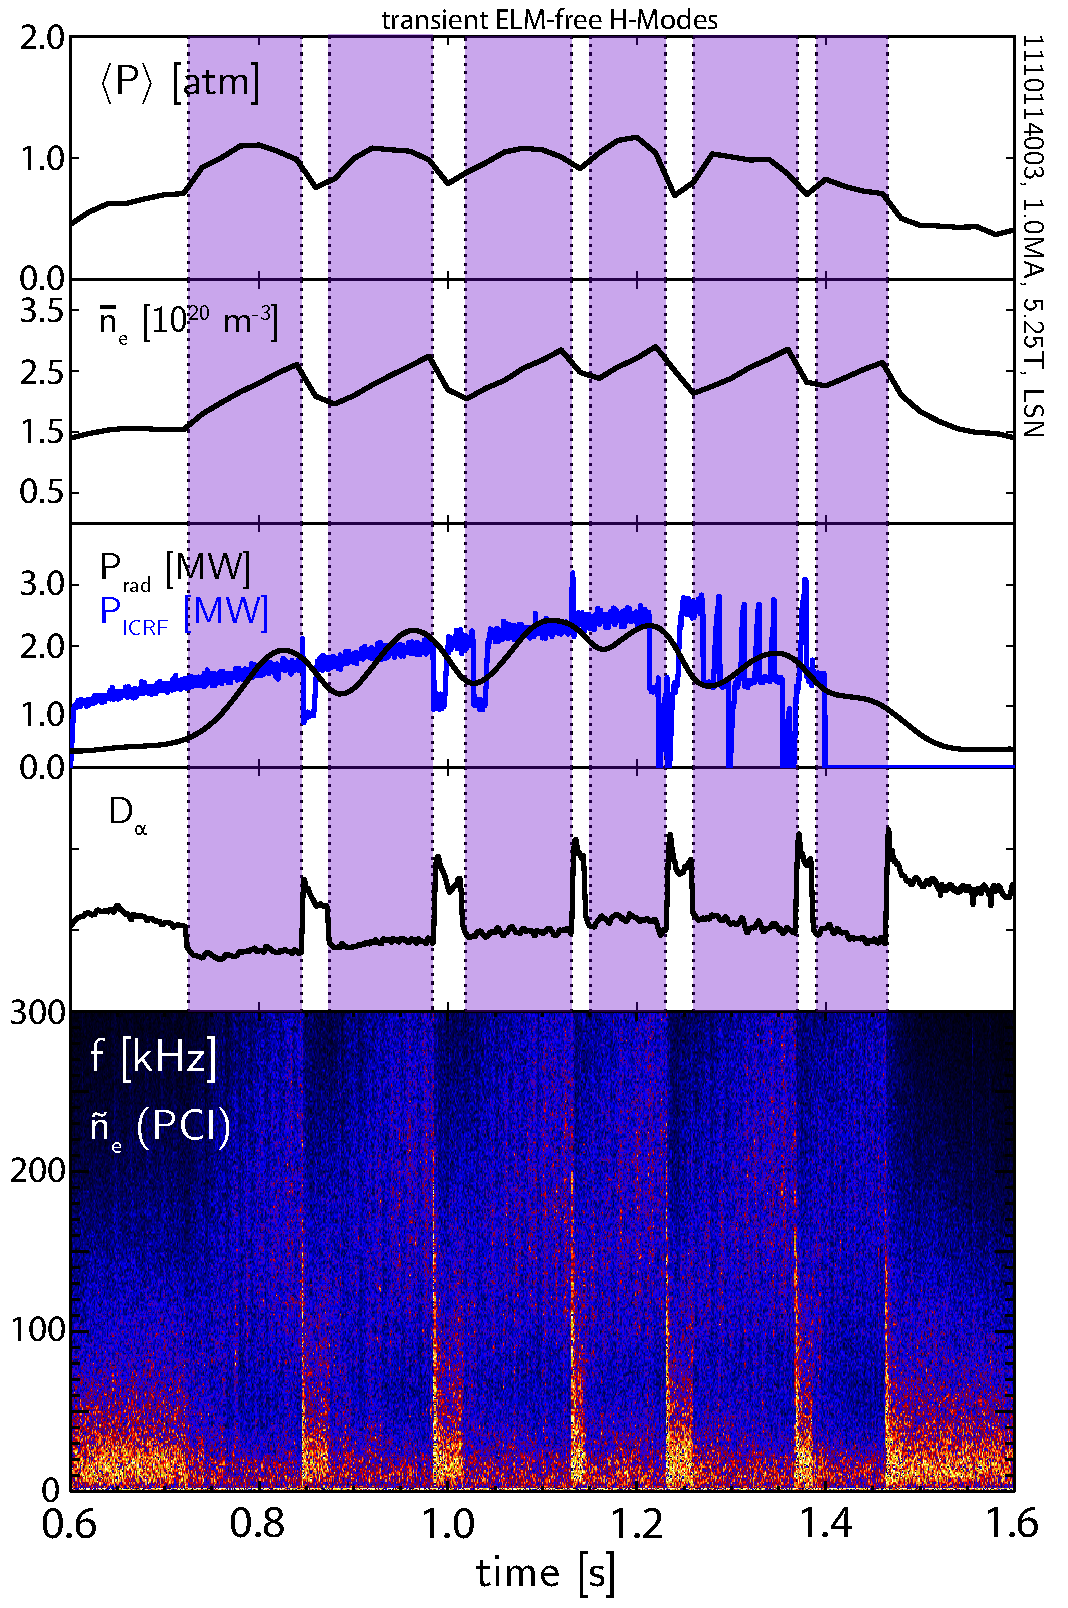
\includegraphics[width=0.85\columnwidth]{graphics/HighPerformanceRegimes/trace_1110114003.pdf}
 \end{columns}

\end{frame}

%%%%%%%%%%%%%%%%%%%%%%%%%%%%%%%%%%%%%%%%%%%%%%%%%%%%%%%%%%%%%%%%%%%%%

\begin{frame}

\Large
so, we need:
\begin{itemize}
 \item high energy confinement
 \item low particle confinement (low enough, at least)
 \item ... and that's it, right?
\end{itemize}

\end{frame}

%%%%%%%%%%%%%%%%%%%%%%%%%%%%%%%%%%%%%%%%%%%%%%%%%%%%%%%%%%%%%%%%%%%%%

\begin{frame}{The solution? (part II)}

 \begin{columns}[c]
  \column{0.5\textwidth}
  \begin{itemize}
   \large
   \item Edge-Localized Modes (ELMs) -- instabilities that relax the pedestal, drive bursts of energy, particle transport, enough to prevent impurity accumulation
   \vspace{0.5em}
   \onslide<2>{\item \textcolor{red}{large ELMs drive pulsed heat loads in excess of plasma-facing material tolerances}}
  \end{itemize}
  \column{0.5\textwidth}
  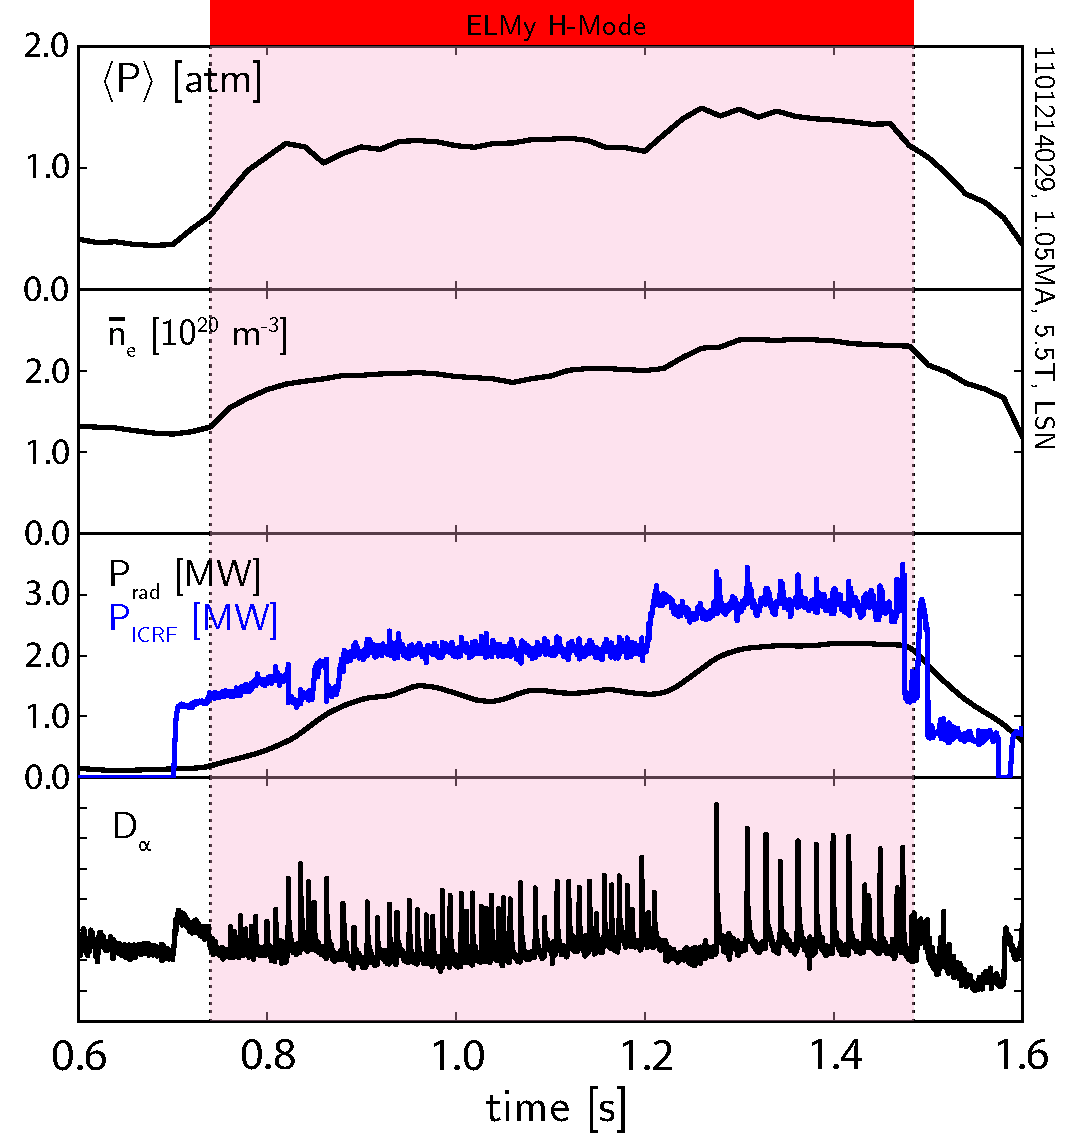
\includegraphics[width=\columnwidth]{graphics/HighPerformanceRegimes/trace_1101214029.pdf}
 \end{columns}

\end{frame}

%%%%%%%%%%%%%%%%%%%%%%%%%%%%%%%%%%%%%%%%%%%%%%%%%%%%%%%%%%%%%%%%%%%%%

\begin{frame}

\Large
so, we need:
\begin{itemize}
 \item high energy confinement
 \item low particle confinement (low enough, at least)
 \item avoid, mitigate, or suppress large ELMs
\end{itemize}

\onslide<2>{\begin{emphblock}{}
  \centering
  Both engineering and physics solutions exist, including...
 \end{emphblock}}

\end{frame}

%%%%%%%%%%%%%%%%%%%%%%%%%%%%%%%%%%%%%%%%%%%%%%%%%%%%%%%%%%%%%%%%%%%%%

\end{document}